\documentclass[10pt]{exam}
\usepackage[icp]{template-for-exam}
\usepackage{tikz}
\usetikzlibrary{arrows.meta}


%\printanswers
\shadedsolutions

\tikzset{f/.append style={-{Stealth[length=3mm,width=2mm]}}}

\newcommand{\hforce}[2]{
  \draw[f] (a) -- ++(#1, 0) 
        node[anchor=south] {#2};
}
\newcommand{\vforce}[2]{
  \draw[f] (a) -- ++(0, #1) 
        node[anchor=west] {#2};
}
\newcommand{\forceblank}{
  \,\fillin[][3em]\SI{}{\newton}
}

\newcommand{\printeqs}{
  \ifprintanswers
  \else
    \begin{center}
      \begin{tabular}{|*8c|}
        \hline 
        && $F_{NET} = ma$ & & & $F_G =mg$ &&\\
        \hline
      \end{tabular}
    \end{center}
  \fi
}

\newcommand{\mypagebreak}{
  \ifprintanswers
  \else
    \pagebreak
  \fi
}

\title{Unit P3 Review (Forces)}
\author{Rohrbach}
\date{\today}

\begin{document}
\maketitle

\printeqs 
\begin{questions}
  \question
    What is true about the net force of an object that is moving forward at a constant speed?

    \begin{solution}[\stretch{1}]
      The net force is zero. \emph{or} The forces are balanced.
    \end{solution}

  \question
    What is true about the net force of an object that is moving forward and speeding up?

    \begin{solution}[\stretch{2}]
      The net force points forward. \emph{or} The forces are unbalanced.
    \end{solution}

    \hrule
    \question
    A car's engine pushes the car forward with a force of 5100 Newtons.  The friction on the car is 1800 Newtons.

    \begin{parts}
      \part
        Draw a free body diagram.
        \begin{subparts}
          \small
          \subpart 
            Make sure all the forces are labeled with letters.
          \subpart
            Put the numbers in the diagram at the proper place
          \subpart
            Draw the direction of the net force and calculate its magnitude
        \end{subparts}

        \begin{solution}[7em]

          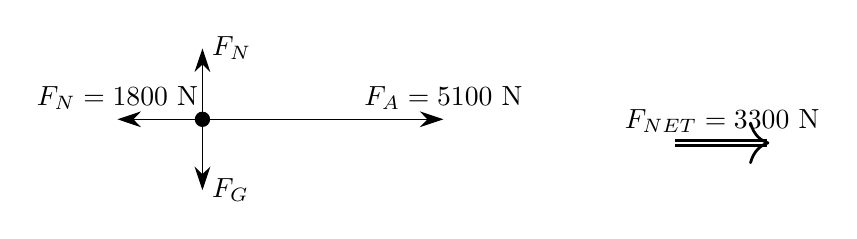
\begin{tikzpicture}[scale=0.6]

            \coordinate (a) at (0,0);
            \filldraw (a) circle [radius=0.15];
            \hforce{5.1}{$F_A=5100$ N}
            \hforce{-1.8}{$F_N=1800$ N}
            \vforce{-1.5}{$F_G$}
            \vforce{1.5}{$F_N$}

            \draw[style=double,line width=1,->] (10,-.5) 
              -- ++(1,0)
              node[anchor=south] {$F_{NET}=3300$ N}
              -- ++(1,0);


          \end{tikzpicture}

        \end{solution}
      

    \part
      The car has a mass of 970 kg.  What is the acceleration of the car?

      \ifprintanswers
        \begin{solution}
          \SI{3.40}{\meter\per\second^2}
        \end{solution}
      \else
        \begin{center}
          \begin{tabular}
            {p{.2\textwidth}|p{.4\textwidth}|p{.2\textwidth}}
            \small Knowns/Unknowns    &
            \small  Plug \& Chug      & 
            \small Answer w/ Units \\
            &&\\[5em]
          \end{tabular}
        \end{center}
      \fi
    \end{parts}
  
  \vspace{1em}

  \hrule

  \question
    What is {\bf inertia} and what law does it correspond to?

    \begin{solution}[\stretch{1}]
      Inertia is the tendency of object's to resist changes in motion.  It corresponds to Newton's First Law.
    \end{solution}
    
  \question
    Which of Newton's laws best explains each of these?  Explain your answer in at least one complete sentence.

    \begin{parts}
      \part 
        Jen goes shopping at the grocery store. She notices that as she adds items to the cart it gets harder to push.   

        \begin{solution}[\stretch{1}]
          Second Law.  As the mass of the cart increases, it accelerates less.
        \end{solution}

      \part 
        A rocket pushes fuel down so that the fuel can push the rocket up.

        \begin{solution}[\stretch{1}]
          Third law.  The action is the rocket pushing the fuel down; the reaction is the fuel pushing the rocket up.
        \end{solution}
    
      \part
        When you are in a car and you slam on your brakes, your body keeps moving forward.

        \begin{solution}[\stretch{1}]
          First law. Your body is in motion.  It tries to stay in motion even though the car stops
        \end{solution}

    \end{parts}

    \question
    You want a 6-kg bowling ball and a 0.5-kg whiffle ball to have the same acceleration.  Which one needs more force?

    \begin{solution}[\stretch{1}]
      The bowling ball needs more force because of the Second Law.  More mass leads to less acceleration, so you need more force to compenate.
    \end{solution}

  \mypagebreak
  \printeqs

  \question
    Identify the Reaction Force in each of these cases:

    \begin{parts}
      
      \part
        You jump off the ground by pushing off of it.  The action force is the force of your feet pushing the ground down.

        \begin{solution}[\stretch{1}]
          The force of the ground pushing your feet up.
        \end{solution}

      \part
        A tennis player hits a ball with his racket.  The action force is the force of the racket pushing the ball forward.

        \begin{solution}[\stretch{2}]
          The force of the ball on the racket.
        \end{solution}
    
    \end{parts}


  
  \hrule

  \question
    A 37-kg crate accelerates at a rate of 2.0 m/s$^2$. 
    
    \begin{parts}
      \part
        Calculate the net force on the crate.

        \ifprintanswers
        \begin{solution}
          $F_{NET}=\SI{74}{\newton}$
        \end{solution}
      \else
        \begin{center}
          \begin{tabular}
            {p{.2\textwidth}|p{.4\textwidth}|p{.2\textwidth}}
            \small Knowns/Unknowns    &
            \small  Plug \& Chug      & 
            \small Answer w/ Units \\
            &&\\[5em]
          \end{tabular}
        \end{center}
      \fi
      
      \part
        Assume that the net force is in the forward direction.  Fill in the blanks in the following free-body diagram

        \begin{center}
          \begin{tikzpicture}[scale=0.7]

            \coordinate (a) at (0,0);
            \filldraw (a) circle [radius=0.15];
            \hforce{5}{$F_A=150$ N}
            \vforce{-1.5}{$F_G=363$ N}

            \ifprintanswers
              \hforce{-2.5}{$F_f=76$ N}
              \vforce{1.5}{$F_N=363$ N}
            \else
              \hforce{-2.5}{$F_f=$\forceblank}
              \vforce{1.5}{$F_N=$\forceblank}
            \fi

          \end{tikzpicture}
        \end{center}

    \end{parts}

  \hrule



  \question
    What is the difference between mass and weight?

    \begin{solution}[\stretch{1}]
      \begin{itemize}
        \item mass is a measure of an object's inertia
        \item weight is the force of gravity on the object
      \end{itemize}
    \end{solution}


	\question 
    If you go to a different planet, what happens to your mass and your weight?

    \begin{solution}[\stretch{2}]
      Your mass stays the same, but your weight changes.
    \end{solution}

  \hrule

  \question
    Consider a 12-kg bowling ball.
	  \begin{parts}
      \part
        What is the bowling ball's weight on earth?
        
        \ifprintanswers
          \begin{solution}
            \SI{117.6}{\newton}
          \end{solution}
        \else
          \begin{center}
            \begin{tabular}
              {p{.2\textwidth}|p{.4\textwidth}|p{.2\textwidth}}
              \small Knowns/Unknowns    &
              \small  Plug \& Chug      & 
              \small Answer w/ Units \\
              &&\\[5em]
            \end{tabular}
          \end{center}
        \fi

      \part
    	  What is the bowling ball's weight on Mars where $g=\SI{3.71}{\meter\per\second^2}$?

        \ifprintanswers
          \begin{solution}
            \SI{44.52}{\newton}
          \end{solution}
        \else
          \begin{center}
            \begin{tabular}
              {p{.2\textwidth}|p{.4\textwidth}|p{.2\textwidth}}
              \small Knowns/Unknowns    &
              \small  Plug \& Chug      & 
              \small Answer w/ Units \\
              &&\\[4em]
            \end{tabular}
          \end{center}
        \fi
    	
    \end{parts}

  \pagebreak
  \printeqs

  \question
    A rocket has a mass of 430 kg.  

    \begin{parts}
      \part
        Calculate the weight (that is, Force of Gravity) of the rocket.

        \ifprintanswers
        \begin{solution}
          \SI{4214}{\newton}
        \end{solution}
        \else
          \begin{center}
            \begin{tabular}
              {p{.2\textwidth}|p{.4\textwidth}|p{.2\textwidth}}
              \small Knowns/Unknowns    &
              \small  Plug \& Chug      & 
              \small Answer w/ Units \\
              &&\\[6em]
            \end{tabular}
          \end{center}
        \fi

      \part 	
        Its engines apply an upward force of 5600 Newtons.  Assume there is no air resistance.  Draw a free body diagram.
        \begin{subparts}
          \small
          \subpart 
            Make sure all the forces are labeled with letters.
          \subpart
            Put the numbers in the diagram at the proper place
          \subpart
            Draw the direction of the net force and calculate its magnitude
        \end{subparts}
        \begin{solution}[10em]
          
          \begin{center}
            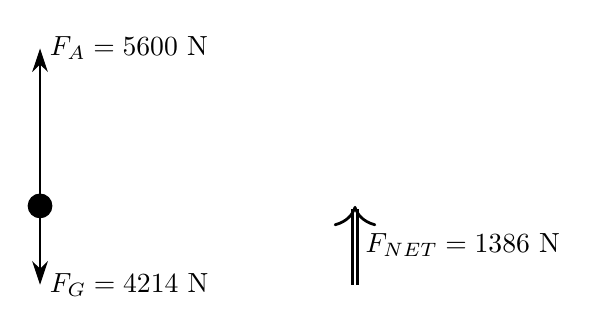
\begin{tikzpicture}

              \coordinate (a) at (0,0);
              \filldraw (a) circle [radius=0.15];
              \vforce{-1}{$F_G=4214$ N}
              \vforce{2}{$F_A=5600$ N}

              \draw[style=double,line width=1,->] (4,-1) 
                -- ++(0,0.5)
                node[anchor=west] {$F_{NET}=1386$ N}
                -- ++(0,0.5);

            \end{tikzpicture}
          \end{center}

        \end{solution}

      \part
        The rocket has a mass of 430 kg.  What is the acceleration of the rocket?

        \ifprintanswers
          \begin{solution}
            \SI{3.22}{\meter\per\second^2}
          \end{solution}
        \else
          \begin{center}
            \begin{tabular}
              {p{.2\textwidth}|p{.4\textwidth}|p{.2\textwidth}}
              \small Knowns/Unknowns    &
              \small  Plug \& Chug      & 
              \small Answer w/ Units \\
              &&\\[6em]
            \end{tabular}
          \end{center}
        \fi


    \end{parts}
    





 

\end{questions}

\end{document}